\documentclass[a4paper]{article}
\usepackage[polish]{babel}
\usepackage[utf8]{inputenc}
\usepackage{polski}
\usepackage[T1]{fontenc}
\frenchspacing
\usepackage{indentfirst}
\usepackage{graphicx} % Required for inserting images
\graphicspath{{./pictures/}}


\begin{document}
\section{Paweł Rycerz}
\label{sec:prycerz}



\[
F(x) = \int_{a}^{b} f(x) \, dx
\]


Oto moje zdjęcie galaktyki (patrz Rysunek~\ref{fig:galaktyka}):
\begin{figure}[h]
    \centering
    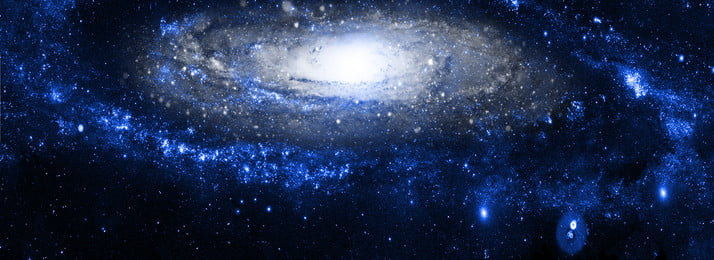
\includegraphics[width=0.25\textwidth]{pictures/galaktyka.png}
    \caption{Podpis do zdjęcia.}
    \label{fig:galaktyka}
\end{figure}


Tabela~\ref{tab:pawel_rycerz} reprezentuje budowe przykładowej tabeli.\\
(To jest moja tabela :D) \\
\begin{table}[h]
    \centering
    \begin{tabular}{|c|c|}
        \hline
        Kolumna 1 & Kolumna 2 \\
        \hline
        Wiersz 1 & Wartość 1 \\
        Wiersz 2 & Wartość 2 \\
        \hline
    \end{tabular}
    \label{tab:pawel_rycerz}
    \caption{Tutaj jest podpis do tabeli.}
\end{table}


Oto przykłady listy numerowanej:

\begin{enumerate}
    \item Pierwszy punkt w liście numerowanej.
    \item Drugi punkt w liście numerowanej.
\end{enumerate}

I listy nienumerowanej:

\begin{itemize}
    \item To jest punkt w liście nienumerowanej.
    \item To jest kolejny punkt w liście nienumerowanej.
\end{itemize}


Oto przykład krótkiego tekstu z podstawowym formatowaniem.\\ \textbf{Ten tekst jest pogrubiony}, \emph{a ten jest kursywą}, \MakeUppercase{a ten tekst jest napisany samymi grubymi literami.}\\

\end{document}